\documentclass{article}
\usepackage{fancyhdr}
\usepackage{graphicx}
\pagestyle{fancy}
\usepackage{geometry}
\usepackage{listings}
\usepackage{enumitem}
\usepackage{color}
\usepackage{fontspec}
\geometry{a4paper, scale=0.75}
\lhead{Yangzhe Xie}
\chead{SWEN90006: Assignment 1}
\rhead{1029787}
\renewcommand{\headrulewidth}{0.4pt}
\renewcommand{\headwidth}{\textwidth}
\definecolor{keywordcolor}{rgb}{0.8,0.1,0.5}
\definecolor{webgreen}{rgb}{0,.5,0}
\definecolor{bgcolor}{rgb}{0.92,0.92,0.92}
\lstset{language=[AspectJ]Java,
    %backgroundcolor=\color{bgcolor}, 设置背景色
    basicstyle=\small,
    commentstyle=\color{blue} \textit, 
    showstringspaces=false,
    captionpos=b,
    xleftmargin=2em,
    xrightmargin=2em, 
    aboveskip=1em
    %numbers=left,
    %numberstyle=\small
}

\title{SWEN90006: Assignment 1}
\author{Name: Yangzhe Xie\\Student number: 1029787\\Email: yangzhe.xie@student.unimelb.edu.au}

\date{\today}
\begin{document}

\maketitle
\thispagestyle{fancy}

\section{Task 1}
\subsection{Test template trees}
Figure 1 - 4 shows the test template trees for the API addUser, loginUser, updateDetails, and retrieveDetails respectively.
\begin{figure}[hbt!]        
\center{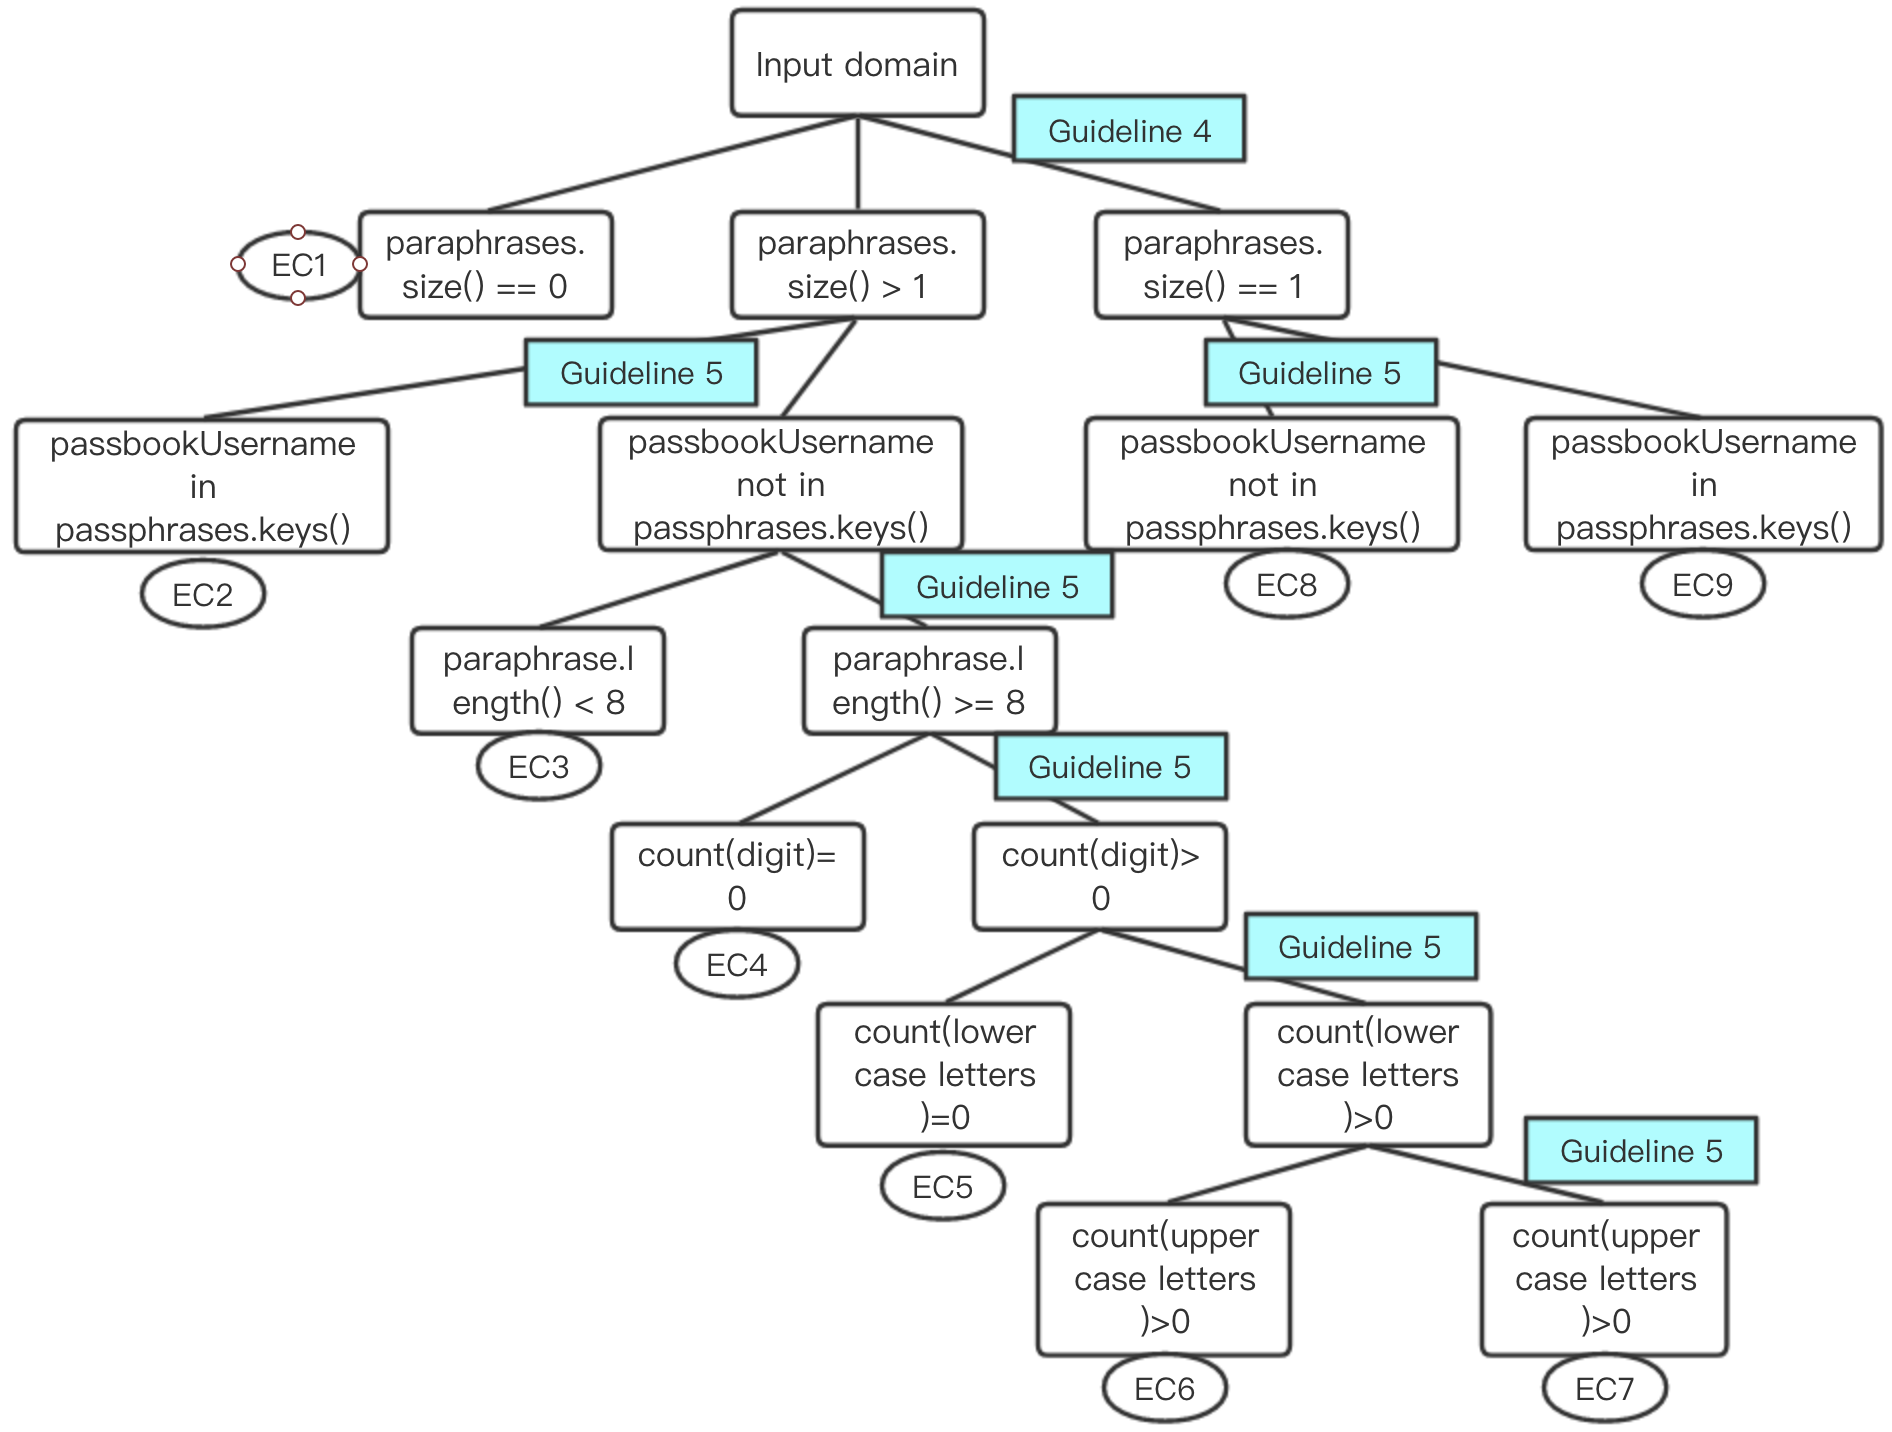
\includegraphics[width=15cm]  {addUser.png}}        
\caption{\label{1} Test template tree for addUser()}      
\end{figure}
\begin{figure}[hbt!]        
\center{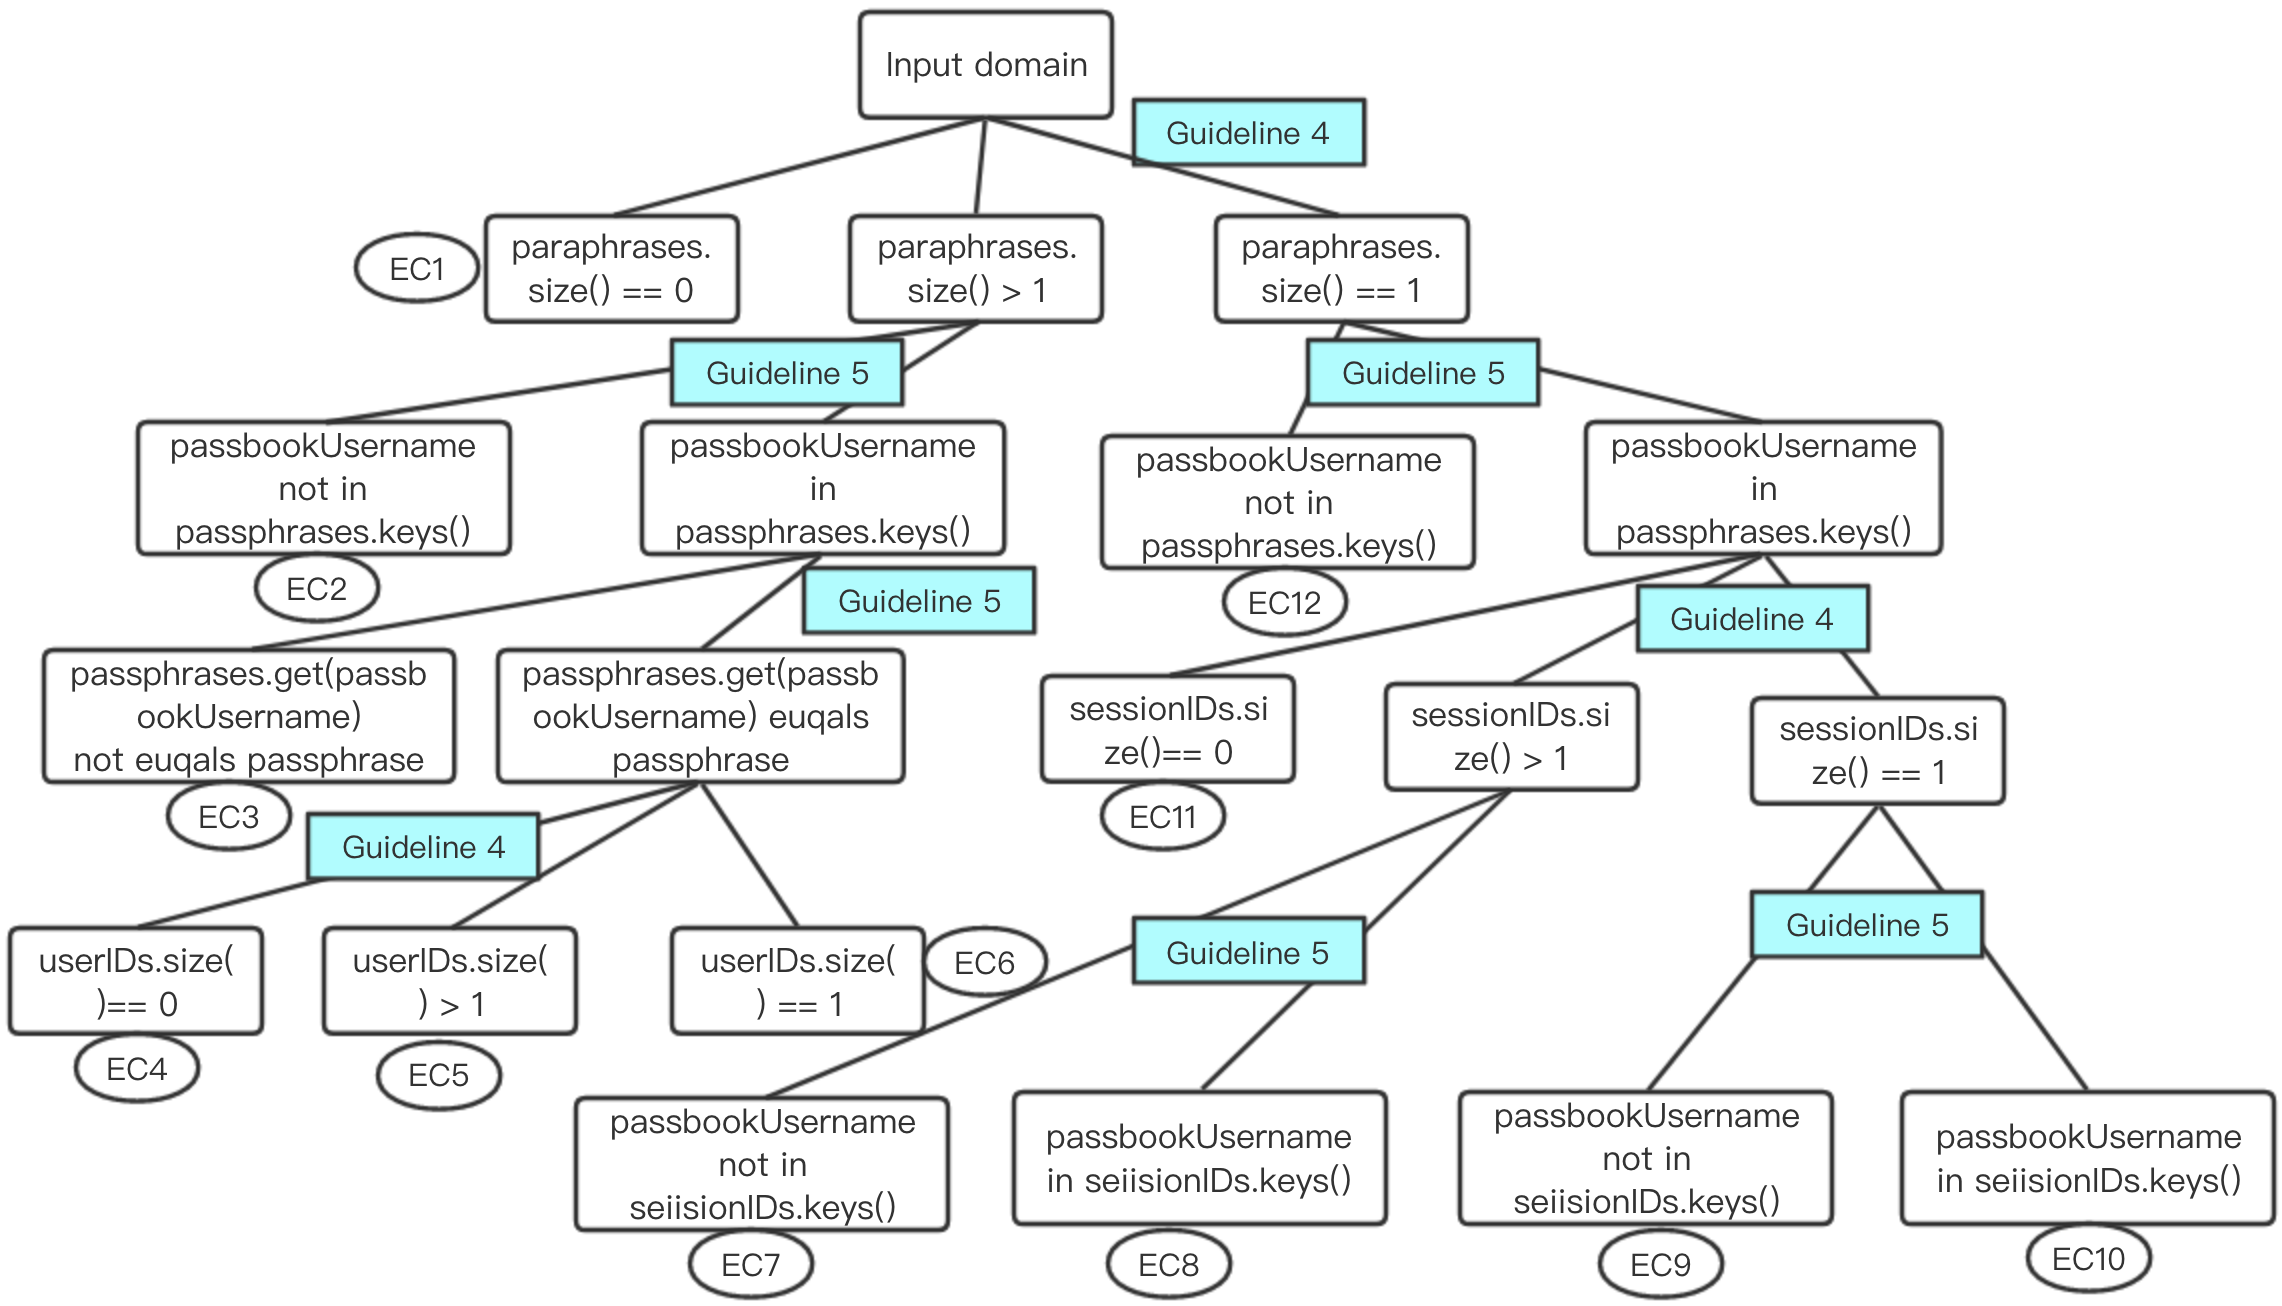
\includegraphics[width=16cm]  {loginUser.png}}        
\caption{\label{1} Test template tree for loginUser()}      
\end{figure}
\begin{figure}[hbt!]        
\center{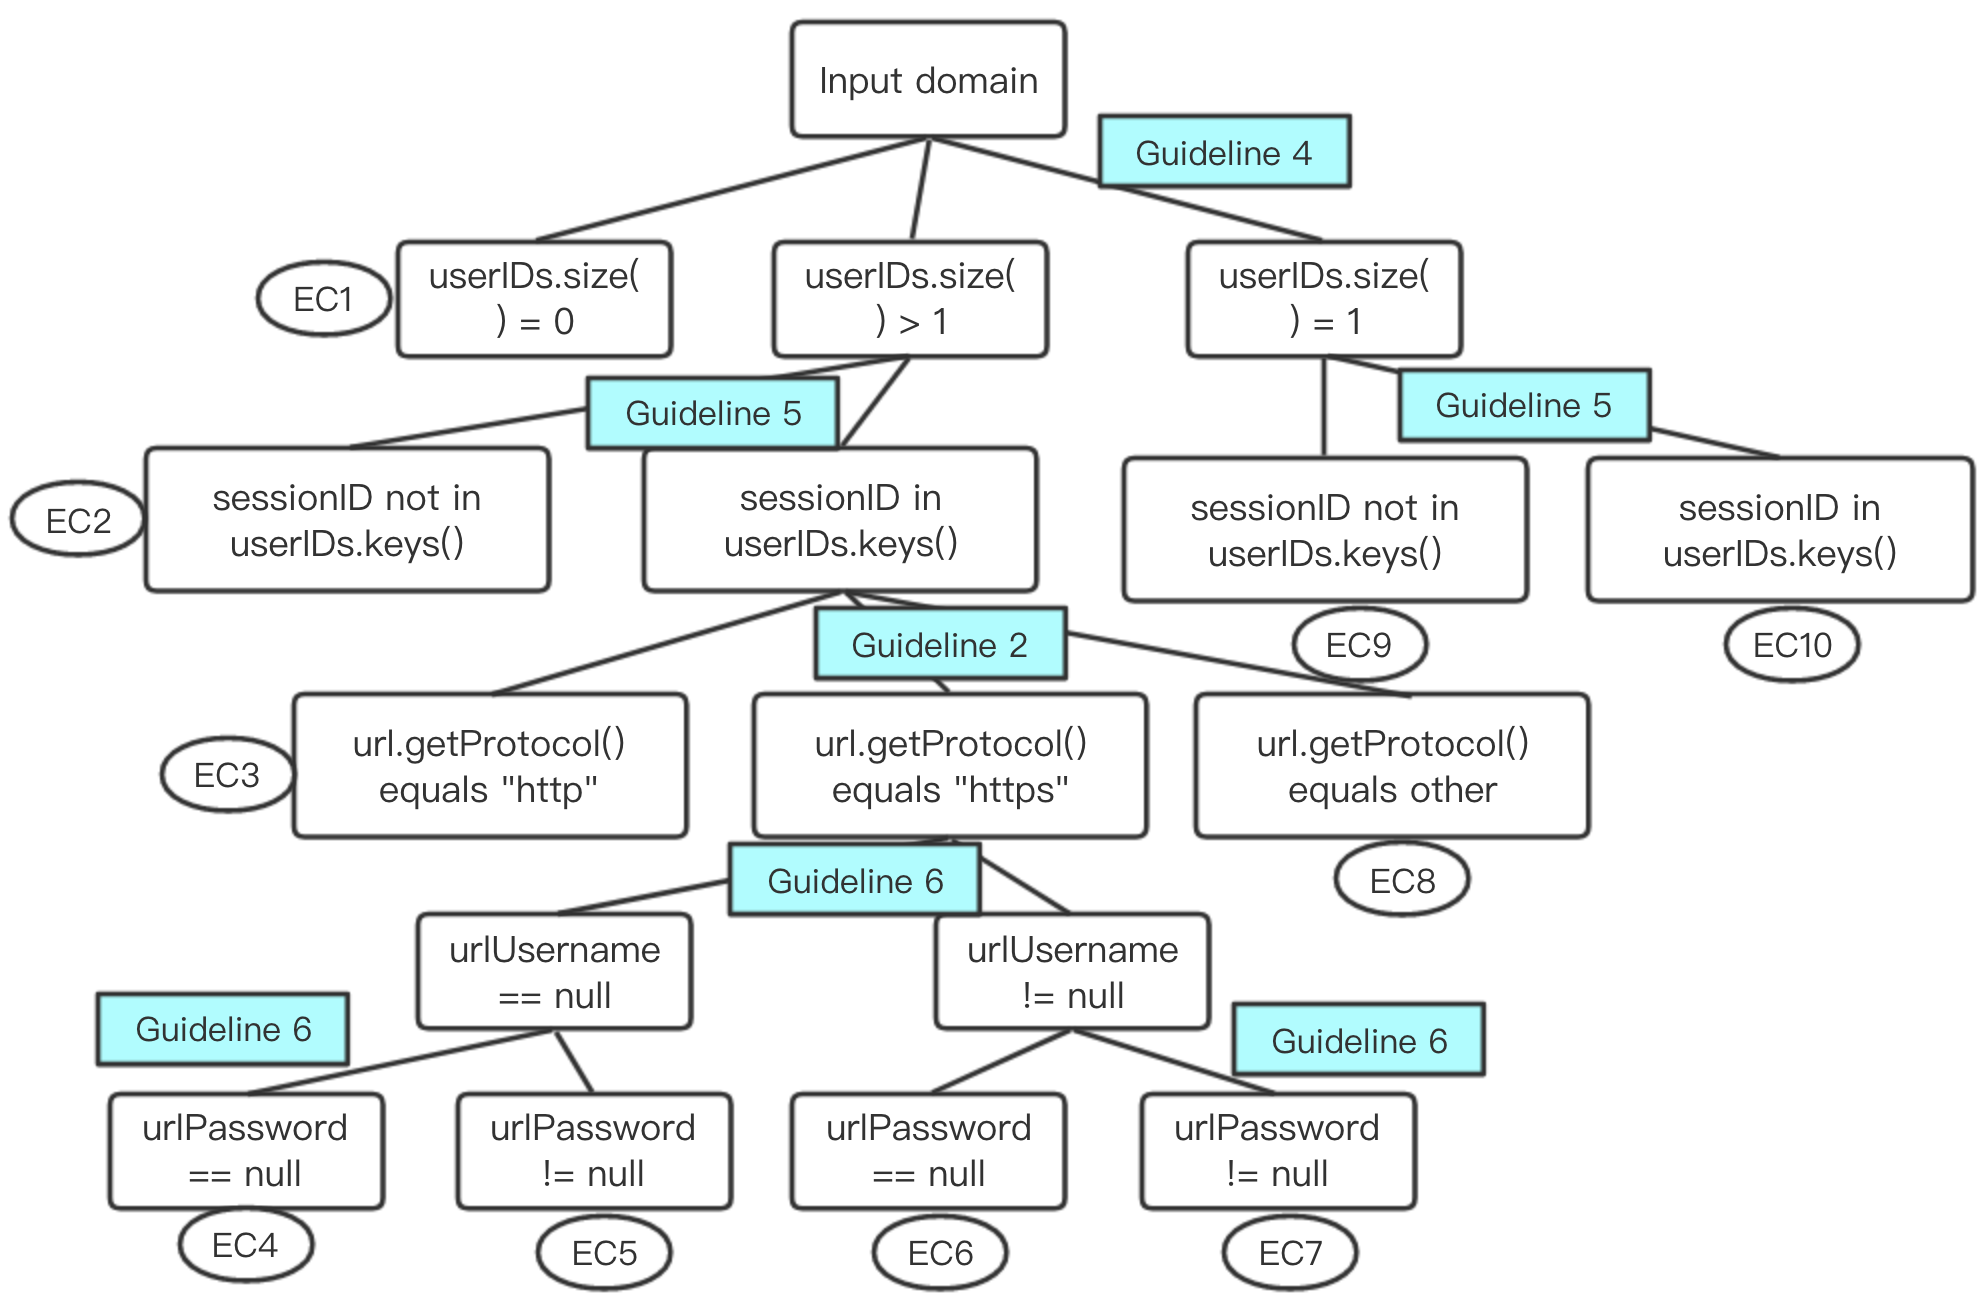
\includegraphics[width=15cm]  {updateDetails.png}}        
\caption{\label{1} Test template tree for updateDetails()}      
\end{figure}
\begin{figure}[t!]        
\center{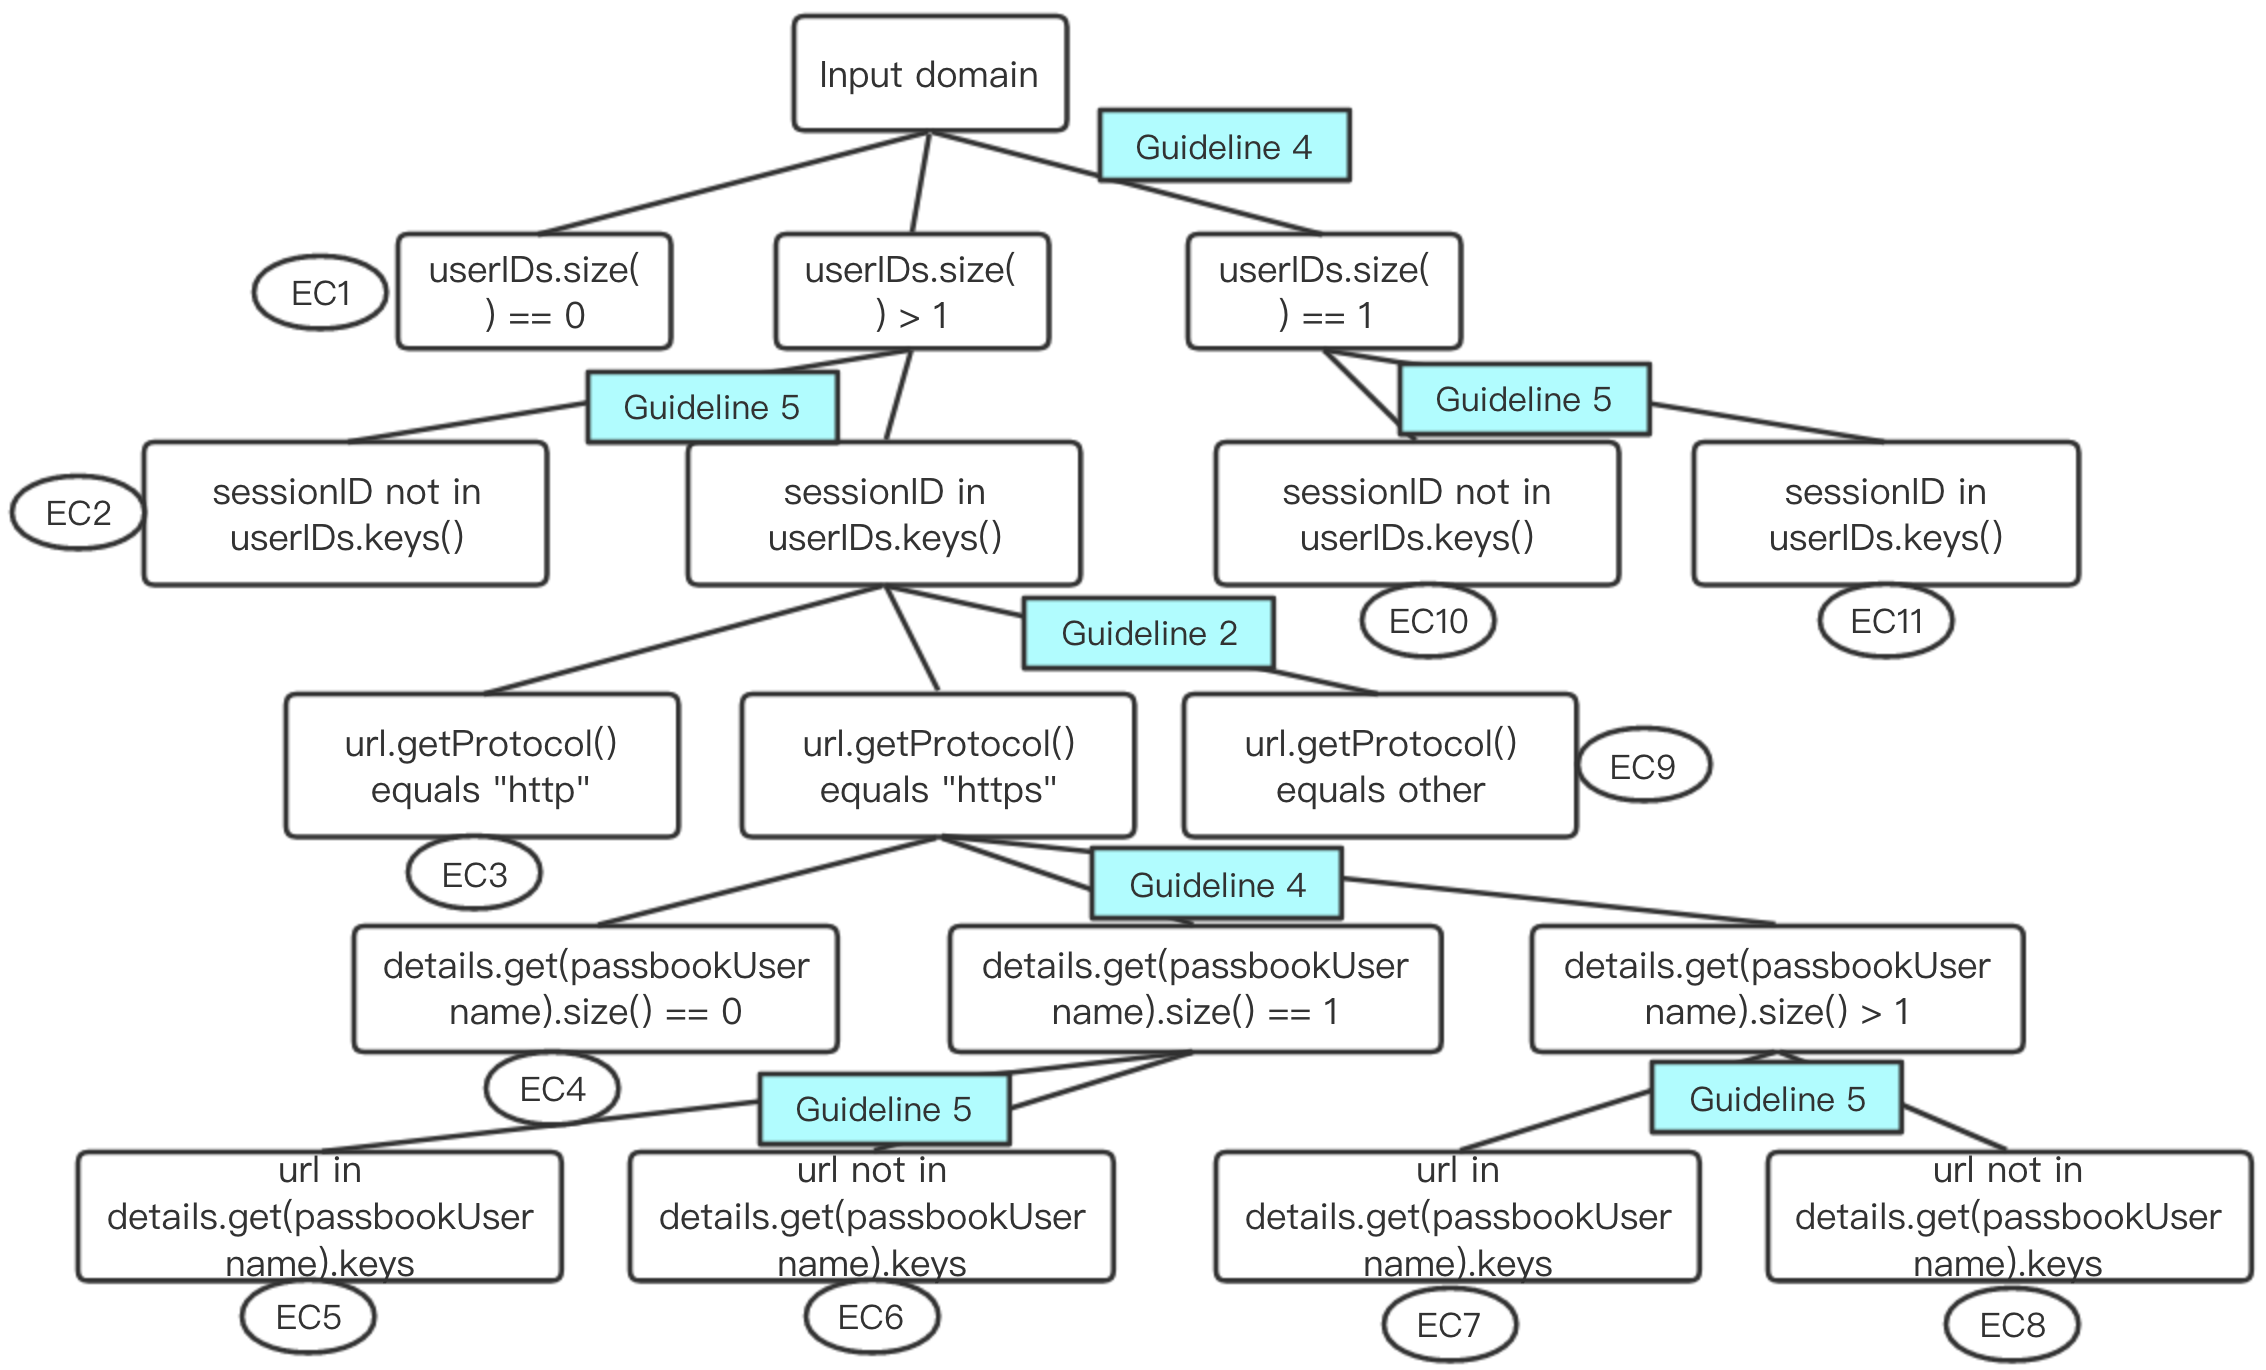
\includegraphics[width=16cm]  {retrieveDetails.png}}        
\caption{\label{1} Test template tree for retrieveDetails()}      
\end{figure}

\subsection{Do your set of equivalence classes cover the input space?}
My set of equivalence classes cover the input space. The reasons are as follows:
\begin{itemize}
\item [1)] All leaf nodes are divided strictly and carefully, so that they do not overlap with other leaf.
\item [2)] The collection of the set of each sibling node covers all the cases of their parent node.
\item [3)]
If two variables are independent of each other, then the subtree of one variable can be added to a leaf node of the other variable. In this case, all the nodes add up to cover all situations.
\item [4)]
As part of your input domain, the instance variables should also be considered. Note that all of these variables are collections, so according to guideline 4, we should follow the zero-one-many rule. But in this particular case, we just care about whether the collection contains some values. So I combined the two cases (number of elements equals 1 and greater than 1) into one (greater than 0), which does not affect the results of the tests.
\end{itemize}
\enddocument